\chapter{Model Compression}
When developing a Deep Neural Network model, it is crucial to consider the devices
on which it will run, especially if the model is to be distributed to users. For
example, running a large language model (LLM) on a mobile device would not be
practical. Therefore, it's important to find the right balance between performance
and compatibility. One possible solution is to host the model in the cloud, but
this approach introduces challenges, such as network latency and privacy concerns.

An alternative approach is to create a more compact model that can run efficiently
on a mobile device while achieving performance similar to that of larger models.
An added advantage of this solution is that, due to its reduced size, the inference
process will be faster.

To achieve these results, several aspects were studied, between the main approaches
we can mention: weight sharing, network pruning, low rank matrix and tensor decomposition,
knowledge distillation, quantization, and low resource and efficient architectures.

\section{Weight Sharing}
\textbf{Weight sharing} is a simple form of network reduction that involves
sharing weights between layers or structures within layers. Unlike other
compression techniques, weight sharing is typically applied before training the
original network, rather than compressing the model after training. This technique
reduces the network size and avoids sparsity. However, it is not always clear
how many and which weights should be shared before performance degradation becomes
unacceptable for a given network architecture and task.

An example of weight sharing can be seen in Convolutional layers, where each
neuron shares the same set of weights across different spatial locations.

\section{Network pruning}
\textbf{Pruning} weights is one of the most commonly used techniques to reduce
the number of parameters in a pre-trained Deep Neural Network. This can lead to
reductions in storage and model runtime. Performance is usually maintained by
retraining the pruned network.

\begin{figure}[!ht]
    \centering
    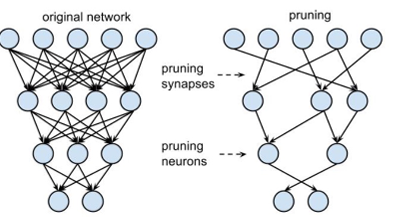
\includegraphics[width=0.5\linewidth]{img/ModelCompression/NetworkPruning.png}
    \caption{Pruning weights in a neural network}
    \label{fig:pruning}
\end{figure}

\textbf{Iterative weight pruning} prunes weights while retraining the network
until the desired trade-off between network size and accuracy is achieved. The
simplest pruning strategy involves setting a threshold to determine which weights
or units (in this case, the absolute sum of the magnitudes of incoming weights)
are removed. The threshold can vary for each layer or be global for the entire
network. Instead of setting a threshold, one can predefine a percentage of weights
to be pruned based on their magnitude, or a percentage aggregated by weights for
each layer. Typically, the weights with magnitudes closest to 0 are removed.

\textbf{Magnitude-based pruning (MBP)} is the most commonly used pruning technique
in DNNs due to its simplicity. It works well for a wide range of machine learning
models, including DNNs, across various tasks. In general, global MBP tends to
outperform layer-wise MBP because it provides more flexibility in determining
the amount of sparsity for each layer. This allows more important layers to remain
denser while less important layers contain more non-zero entries.

\subsection{Categorization of Pruning Techniques}
\begin{itemize}
    \item \textbf{Magnitude-based (iterative pruning + retraining)}: This technique
          removes the weights with the lowest absolute values based on a set
          threshold or percentage, either layer-wise or globally. The steps are
          as follows:
          \begin{enumerate}
              \item Choose a neural network architecture.
              \item Train the network until a reasonable solution is obtained.
              \item Prune the weights with magnitudes smaller than a threshold $\tau$.
              \item Retrain the network until a reasonable solution is obtained.
              \item Repeat step 3.
          \end{enumerate}
    \item \textbf{Methods that penalize the objective} with a regularization
          ($L_1$, $L_2$, etc.) term to force the model to learn a network with
          smaller weights and prune the smallest weights.

          This pruning technique is based on weight regularization, where we add
          a penalty term to the objective function to encourage the model's weights
          to approach zero. The smallest weights are then deleted.

          Typically, an $L_2$ regularization is used:
          \begin{equation*}
              C(\textbf{w}, \textbf{v}) = \frac{\varepsilon}{2} \left(\sum_{m = 1}^h \sum_{l =  1}^n \textbf{w}_{ml}^2 + \sum_{m = 1}^h \sum_{p =  1}^C \textbf{v}_{pm}^2\right)
          \end{equation*}
          However, the main issue with using the above quadratic penalty is that
          all parameters decay exponentially at the same rate and disproportionately
          penalizes larger weights.
    \item \textbf{Methods that compute the sensitivity of the loss function} when
          weights are removed, using this sensitivity as a criterion for removing
          weights that result in the smallest change in loss. \textbf{(Diagonal)
              Hessian-based pruning: Optimal Brain Damage}:
          \begin{enumerate}
              \item Choose a neural network architecture.
              \item Train the network until a reasonable solution is obtained.
              \item Compute the second derivatives for each parameter.
              \item Compute the saliencies for each parameter: $S_k = \frac{\delta^2E}{\delta^2 u_k} u_k^2$.
              \item Sort the parameters by saliency and delete low-saliency parameters.
              \item Repeat step 2.
          \end{enumerate}
    \item \textbf{Search-based approaches} (e.g particle filters, evolutionary
          algorithms, reinforcement learning) that seek to learn or adapt a set
          of weights, links, or paths within the neural network, keeping those
          that are salient for the task.
\end{itemize}
\subsection{Structured vs. Unstructured Pruning}
Another important distinction to be made is between structured and unstructured
pruning techniques:
\begin{itemize}
    \item \textbf{Structured pruning} aims to preserve network density for
          computational efficiency (resulting in faster computation at the expense
          of less flexibility) by removing groups of weights.
    \item \textbf{Unstructured pruning} is unconstrained as to which weights or
          activations are removed, but the sparsity means that the dimensionality
          of the layers does not change.
\end{itemize}
Therefore, sparsity in unstructured pruning techniques generally provides good
performance at the expense of slower computation.

\subsubsection{Structured pruning via weight regularization}
Since standard pruning leads to non-structured connectivity, structured pruning
can be used to reduce memory usage and increase speed. Hardware is more amenable
to dealing with dense matrix multiplications, especially when there are few
non-zero entries in matrices and tensors. Convolutional Neural Networks (CNNs)
are particularly suitable for this type of pruning since they consist of sparse
connections.

\subsubsection{Group sparsity regularization}
Group sparse regularizers enforce a subset of weight groupings (such as filters
in CNNs) to be close to zero when trained using stochastic gradient descent. For
example, consider a convolutional kernel represented as a tensor $K(i; j; s; :)$.
The group-wise $L_1$-norm, $L_2$-norm is given as:
\begin{equation*}
    \omega_{2, 1}(K) = \lambda \sum_{i, j, s} | \Gamma_{ijs} | = \lambda \sum_{i, j, s} \sqrt{\sum_{t= 1}^T K(i, j, s, t)^2}
\end{equation*}

Where $\Gamma_{ijs}$ is the group of kernel tensor entries $K(i; j; s; :)$, where
$(i;j)$ represents the pixel location in the $i$-th row and $j$-th column of the
image for the $s$-th input feature map. This regularization term forces certain
groups $\Gamma_{ijs}$ to be close to zero, which can be useful for pruning.

\section{Low rank matrix and tensor decomposition}
The idea starts from the observation that most weights are in the fully connected
layers, and that fully connected layers are implemented with a single matrix
multiplication, i.e. connections from a fully connected layer with $N$ units into
one with $M$ units can be stored in a $W = N \times M$ matrix.

Let's now rewrite the matrix $W$ as a product of three matrices $U$, $S$ and $V$:
\begin{equation*}
    W = USV^T
\end{equation*}
where $U \in \mathbb{R}^{m \times m}$ matrix, $S \in \mathbb{R}^{m \times k}$
diagonal matrix and $V \in \mathbb{R}^{k \times k}$ matrix.

By only keeping the $t(< k)$ singular values with largest magnitude:
\begin{equation*}
    \tilde{W} = \tilde{U} \tilde{S} \tilde{V^T}
\end{equation*}
where $U \in \mathbb{R}^{m \times t}$ matrix, $S \in \mathbb{R}^{t \times t}$
diagonal matrix and $V \in \mathbb{R}^{t \times k}$ matrix. So the number of
parameters is reduced from $m \times k$ to $m \times t + t + t \times k$.
\section{Knowledge distillation}
Involves learning a smaller network from a large network using supervision from
the larger network and minimizing the entropy, distance or divergence between
their probabilistic estimates. Probably the first work about KD is from Bucilua
et al. where they explored the idea of reducing model size by learning a student
network from an ensemble of models.
\begin{itemize}
    \item They use a teacher network to label a large amount of unlabeled data
          and train a student network using supervision from the pseudo labels
          provided by the teacher;
    \item They find performance is close to the original ensemble with $1000 \times$
          smaller network.
\end{itemize}

Hinton et al. showed a neural network knowledge distillation approach where a
small model is trained using supervision (class probability outputs) from the
original “teacher” model. They showed that learning from the larger network
outperformed the smaller network learning from scratch in the standard supervised
classification setup.

\begin{figure}[!ht]
    \centering
    \includegraphics[width=0.5\linewidth]{img/ModelCompression/KnowledgeDistillation.png}
    \caption{Knowledge Distillation}
    \label{fig:knowledgeDistillation}
\end{figure}

\section{Quantization}
\textbf{Quantization} is the process of representing values with a reduced number
of bits. In neural networks, this can be applied to weights, activations and
gradient values. Typically, when training on the GPU, values are stored in 32-bit
floating point (FP) single precision. Half-precision for floating point (FP-16)
and integer arithmetic (INT-16) are also commonly considered. INT-16 provides
higher precision but a lower dynamic range compared to FP-16. In FP-16, the result
of a multiplication is accumulated into a FP-32 followed by a down-conversion to
return to FP-16.

To speed up training, faster inference and reduce bandwidth memory requirements,
ongoing research has focused on training and performing inference with lower-precision
networks using integer precision (IP) as low as INT-8, INT-4, INT-2 or 1 bit
representations.

Designing such networks makes it easier to train such networks on CPUs, FPGAs,
ASICs and GPUs. Two important features of quantization are the range of values
that can be represented and the bit spacing.

For the range of signed integers with n bits, we represent a range of $[-2n-1, 2n-2]$
and for full precision (FP-32) the range is $\pm3.4e38$. For signed integers,
there are $2n$ values in that range and approximately $4.2e9$ for FP-32. FP can
represent a large array of distributions which is useful for neural network
computation, however this comes at larger computational costs when compared
to integer values.

For integers to be used to represent weight matrices and activations, a FP scale
factor is often used hence many quantization approaches involve a hybrid of mostly
integer formats with FP-32 scaling numbers. This approach is often referred to
as mixed-precision (MP). Different MP strategies have been used to avoid overflows
during training and/or inference of low resolution networks given the
limited range of integer formats.
\section{Low resource and efficient architectures}
\begin{itemize}
    \item \textbf{MobileNet}: is a sort of compression of CNN for embedded mobile
          vision application. They use depth-wise separable convolution (DSC) and
          2 hyperparameter that trade off latency and accuracy. DSC split the
          convolution in 2 steps, first filtering then combining outputs of each
          DSC filter, this is why it is referred as factorization approach.
          \begin{figure}[!ht]
              \centering
              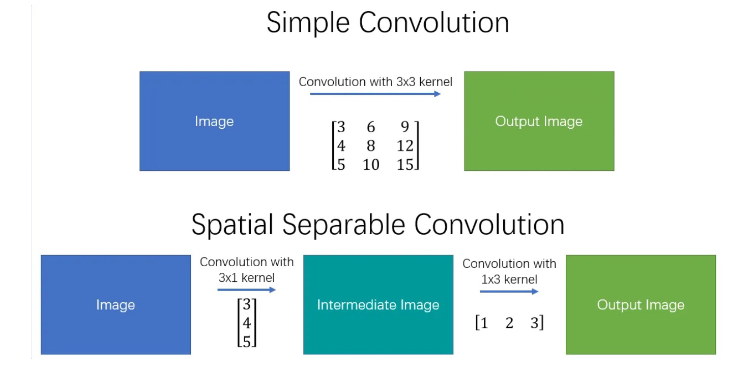
\includegraphics[width=0.5\linewidth]{img/CNN/spatialConv.png}
              \caption{Spatial Separable Convolution}
              \label{fig:spatialConv}
          \end{figure}
    \item \textbf{SqueezeNet}: reduce the network architecture by reducing $3 \times 3$
          filters to $1\times1$ filters (squeeze layer). Reduce the number of
          input channels to $3 \times 3$ filters using squeeze layers and down
          sample later in the network to avoid the bottleneck of information
          through the network too early and in turn lead to better performance.
          A fire module is made up of the squeeze layer and an expand layer that
          is a mix of $1 \times 1$ and $3 \times 3$ convolution filters. The number
          of filters per fire module is increased as it gets closer to the
          last layer.
    \item \textbf{ShuffleNet}: uses point-wise group convolutions (i.e using a
          different set of convolution filter groups on the same input features,
          this allows for model parallelization) and channel shuffles (randomly
          shuffling helps information flow across feature channels) to reduce
          compute while maintaining accuracy. ShuffleNet is made up economical
          $3 \times 3$ depth-wise convolutional filters and replace $1 \times 1$
          layer with point-wise group convolutional followed by the channel
          shuffle. Unlike predecessor models, ShuffleNet is efficient for smaller
          networks.
    \item \textbf{DenseNet}: Gradients can vanish in very deep networks because
          the error becomes more difficult to backpropagate as the number of
          matrix multiplications increases. DenseNets address gradient vanishing
          connecting the feature maps of the previous layer to the inputs of the
          next layer, similar to ResNet skip connections. This reusing of features
          means the network efficient with its use of parameters. Although, deep
          and thin DenseNetworks can be parameter efficient, they do tradeoff
          with memory/speed efficiency in comparison to shallower yet wider network
          because all layer outputs need to be stored to perform backpropagation.
          However, DenseNets too can be made wider and shallower to become more
          memory efficient if required.
\end{itemize}